% generated by experiments/build_paper_assets.py -- do not edit by hand
\begin{figure}[t]
\centering
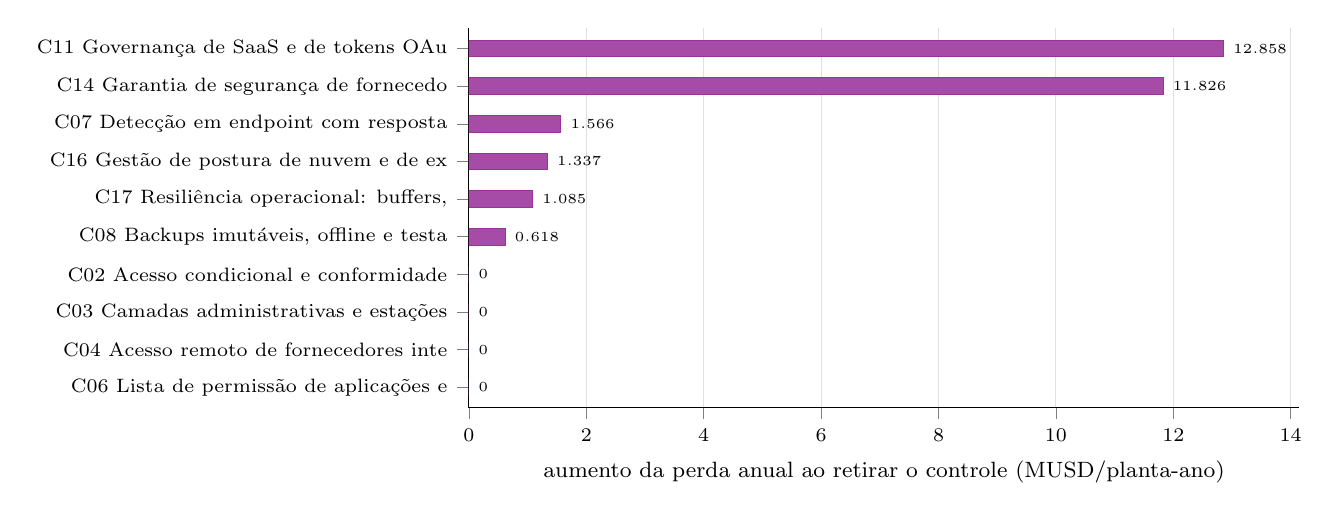
\begin{tikzpicture}
\begin{axis}[
    xbar, width=\linewidth, height=6.4cm,
    xlabel={aumento da perda anual ao retirar o controle (MUSD/planta-ano)},
    xmin=0, enlarge y limits=0.06,
    ytick={0,1,2,3,4,5,6,7,8,9}, yticklabels={{C11 Governança de SaaS e de tokens OAu},{C14 Garantia de segurança de fornecedo},{C07 Detecção em endpoint com resposta },{C16 Gestão de postura de nuvem e de ex},{C17 Resiliência operacional: buffers, },{C08 Backups imutáveis, offline e testa},{C02 Acesso condicional e conformidade },{C03 Camadas administrativas e estações},{C04 Acesso remoto de fornecedores inte},{C06 Lista de permissão de aplicações e}},
    y dir=reverse, ticklabel style={font=\scriptsize},
    label style={font=\footnotesize},
    nodes near coords, nodes near coords style={font=\tiny},
    every node near coord/.append style={/pgf/number format/fixed,
        /pgf/number format/precision=3},
    xmajorgrids, grid style={gray!25}, axis lines*=left,
    bar width=6pt, tick align=outside,
]
\addplot[fill=Purple!70, draw=Purple!80] coordinates {
        (12.858000,0)
        (11.826000,1)
        (1.566000,2)
        (1.337000,3)
        (1.085000,4)
        (0.618000,5)
        (0.000000,6)
        (0.000000,7)
        (0.000000,8)
        (0.000000,9)
};
\end{axis}
\end{tikzpicture}
\caption{Necessidade de cada controle dentro do programa completo $S_5$: a perda anual que retorna quando apenas aquele controle é retirado.}
\label{fig:necessity}
\end{figure}
